\part{Netværk basic}
\chapter{Grundlæggende netværkskommunikation i IoT}
Netværkskommunikation er rygraden i moderne teknologi og især vigtig i konteksten af Internet of Things (IoT) og industriel anvendelse. For at forstå, hvordan enheder kommunikerer, skal vi først forstå de grundlæggende koncepter i netværkskommunikation.
\begin{itemize}
	\item \textbf{Hvad er et netværk?} Et netværk er et sæt af interforbundne enheder (som computere, sensorer, gateways) der kan dele data. Det kan være så simpelt som to computere forbundet via et Ethernet-kabel eller så komplekst som hele internettet.5
	\item \textbf{LAN vs. WAN:} LAN (Local Area Network) er et netværk, der er begrænset til et lille geografisk område, som et kontor eller en bygning. WAN (Wide Area Network) dækker et større geografisk område og kan forbinde byer eller endda lande.
	\item \textbf{Protokoller:} Kommunikation mellem enheder styres af regler kaldet protokoller. De mest kendte protokoller inkluderer TCP/IP, der bruges til at styre dataoverførsel på internettet.
	\item \textbf{IP-adresser og MAC-adresser:} Enhver enhed på et netværk skal have en entydig adresse. IP-adressen er en numerisk adresse, der identificerer en enhed på et netværk, mens MAC-adressen er en hardwareadresse, der er unik for netværksgrænsefladen.
	\item \textbf{Routing og Switching:} Routere og switches spiller en afgørende rolle i, hvordan data dirigeres gennem et netværk. Routere bruges til at forbinde forskellige netværk, mens switches styrer dataflow inden for et enkelt netværk.
	\item \textbf{Sikkerhed:} Netværkssikkerhed er vital, især i industrielle miljøer, hvor et angreb kan føre til alvorlig skade. Det omfatter foranstaltninger som firewall, kryptering og autentifikation.
	\item \textbf{Internet of Things (IoT):} IoT refererer til et netværk af forbundne fysiske enheder, der kan samle og udveksle data. I en industriel kontekst kan dette være sensorer, maskiner og kontrolsystemer, der kommunikerer for at optimere produktion.
	\item \textbf{Kabel vs. Trådløst:} Enheder kan forbindes via kabler (som Ethernet) eller trådløst (som Wi-Fi). Valget afhænger af applikationen og kravene til hastighed, pålidelighed og sikkerhed.
	\item \textbf{Sky og Edge Computing:} Dette refererer til, hvor databehandling sker, enten centralt i skyen eller på kanten af netværket tættere på enhederne.
	\item \textbf{QoS (Quality of Service):} I industrielle netværk er det afgørende at kunne prioritere trafik for at sikre, at vigtige data når frem i tide.
\end{itemize}
Ved at forstå disse grundlæggende koncepter kan man bedre designe, implementere og vedligeholde netværk, der er i stand til at understøtte de unikke krav og udfordringer, der findes i industrielle og IoT-applikationer.

\subsection{Hvad er et netværk?}
Et netværk refererer til en samling af computere, servere, hovedsystemer, netværksenheder, periferiudstyr eller andre enheder, der er forbundet til hinanden, så de kan dele data. Nedenfor er en mere detaljeret forklaring på forskellige aspekter af netværk.
\begin{enumerate}
	\item \textbf{Typer af Netværk}
	\begin{itemize}
		\item \textbf{Lokalt Netværk (Local Area Network - LAN):} Dette er et netværk i en lille geografisk placering som et kontor, bygning eller campus.
		\item \textbf{Bredt Netværk (Wide Area Network - WAN):} WAN forbinder flere LANs, som kan være placeret i forskellige byer eller lande.
		\item \textbf{Personligt Netværk (Personal Area Network - PAN):} Dette er et lille netværk, der bruges til at forbinde personlige enheder som smartphones og bærbare computere.
		\item \textbf{Metropol Netværk (Metropolitan Area Network - MAN):} Et netværk, der dækker en større geografisk placering som en hel by.
	\end{itemize}
	\item \textbf{Netværks Topologier}
	\begin{itemize}
		\item \textbf{Stjerne Topologi:} Hver enhed er forbundet til en central hub eller switch.
		\item \textbf{Ring Topologi:} Enheder er forbundet i en cirkel uden central enhed.
		\item \textbf{Bus Topologi:} Alle enheder deler en enkelt kommunikationslinje.
		\item \textbf{Mesh Topologi:} Enheder er forbundet med mange andre enheder, så der er mange mulige veje for informationen at rejse.
	\end{itemize}
	\begin{figure}[!h]
		\centering
		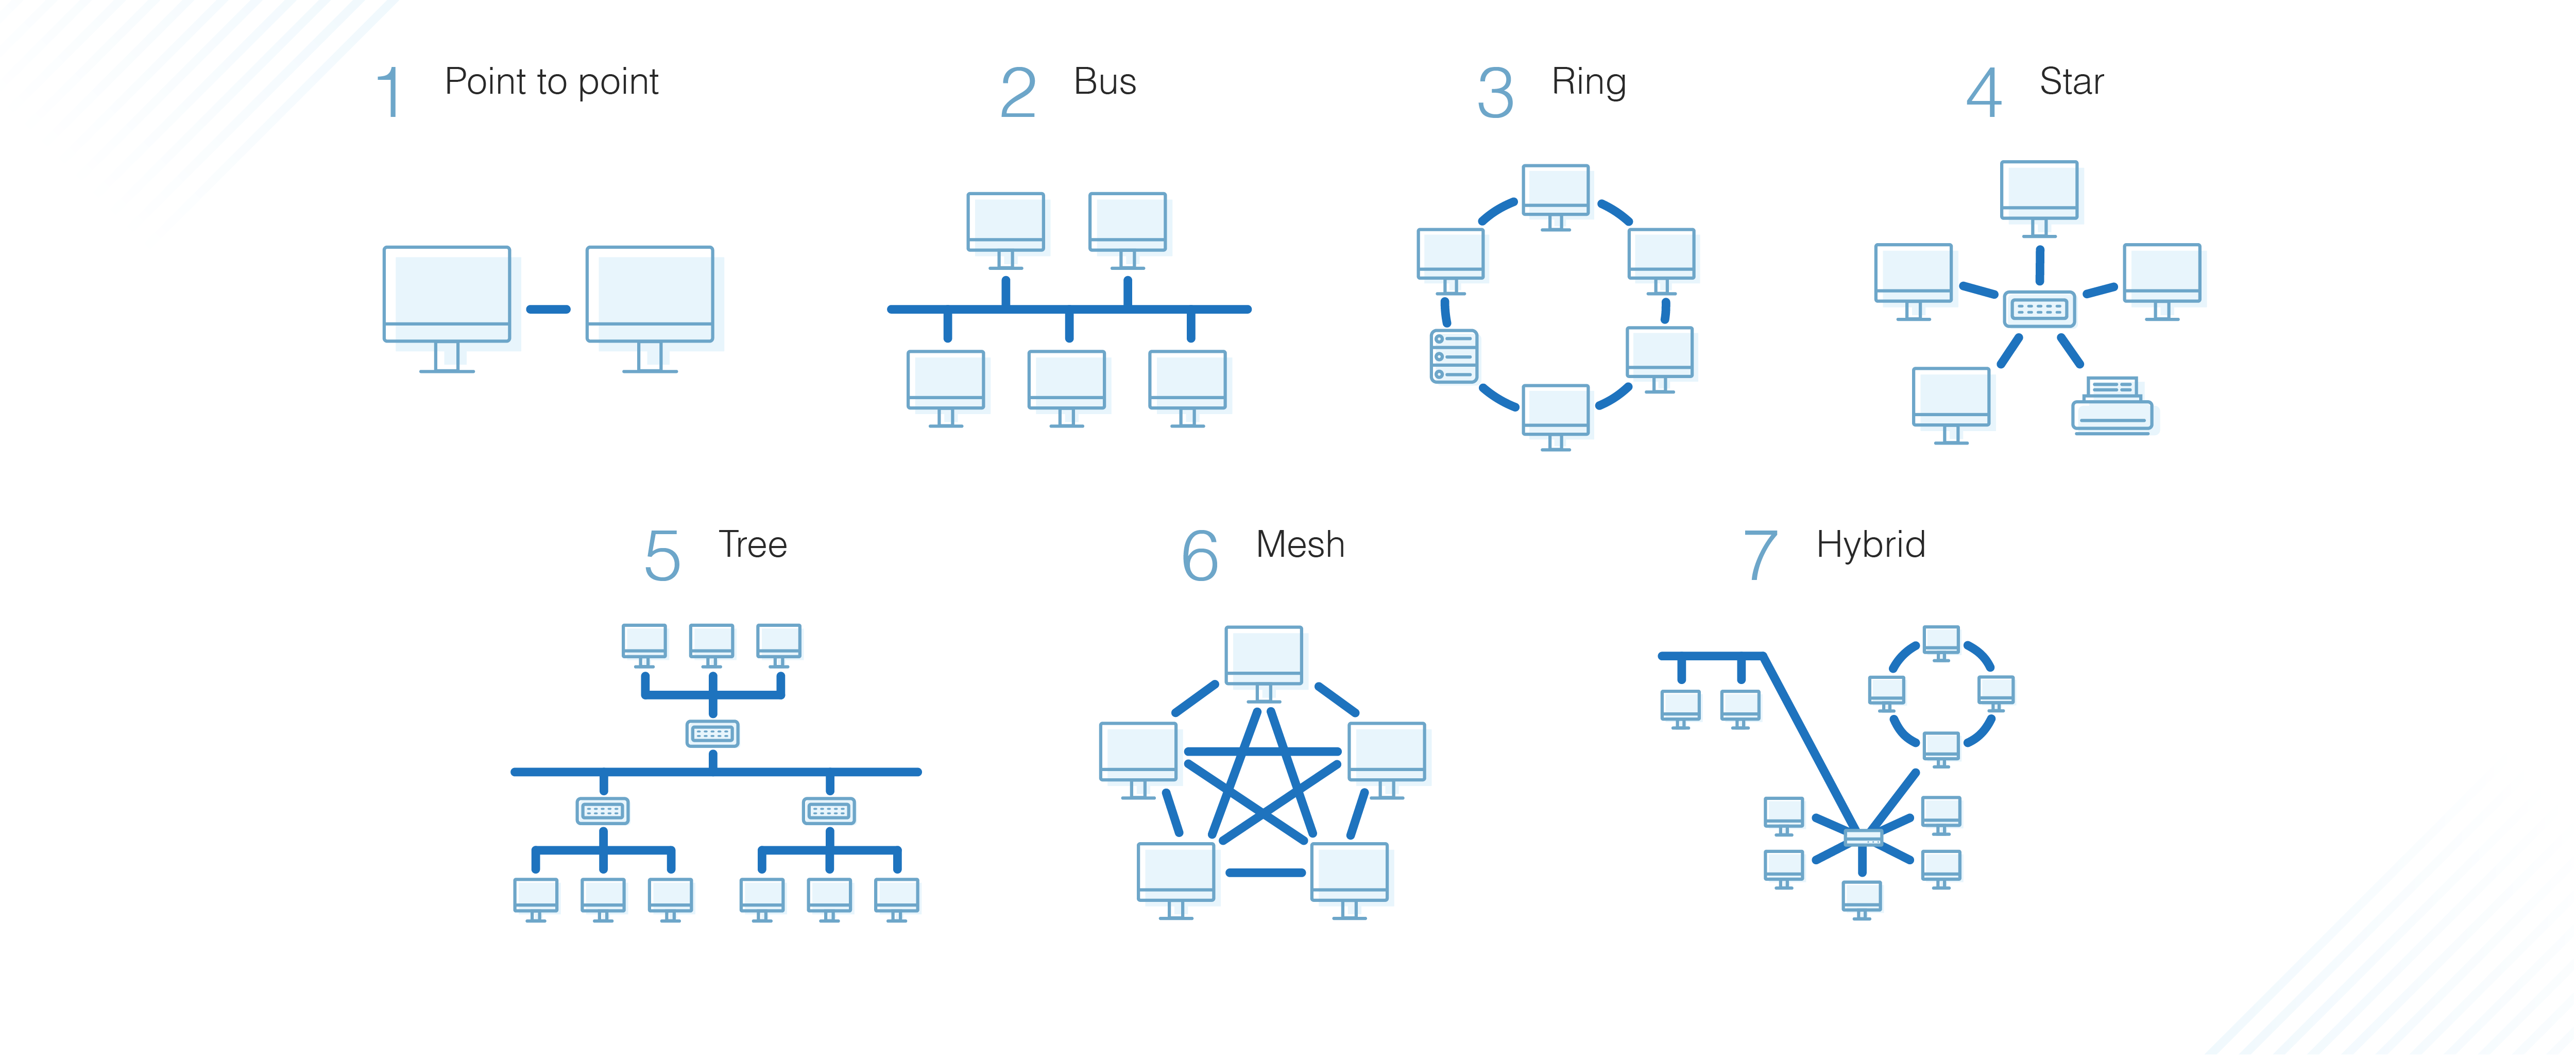
\includegraphics[width=\textwidth]{fig/fig34.png}
	\end{figure}
	\item \textbf{Protokoller og Modeller}
	\begin{itemize}
		\item \textbf{TCP/IP:} Dette er den grundlæggende protokol, der driver internettet, og står for Transmission Control Protocol/Internet Protocol.
		\item \textbf{UDP (User Datagram Protocol):} En lettere, men mindre pålidelig protokol end TCP, brugt til applikationer, hvor hastighed er vigtigere end pålidelighed, såsom videostreaming.
		
		\item \textbf{OSI Model:} OSI-modellen (Open Systems Interconnection) er en referencemodel, der beskriver, hvordan applikationer på netværksenheder skal kommunikere over et netværk.
	\end{itemize}
	\item \textbf{Netværkets Hardware}
	\begin{itemize}
		\item \textbf{Routere:} Disse styrer trafik mellem forskellige subnets og kan forbinde forskellige netværk.
		\item \textbf{Switche:} De bruges til at forbinde enheder inden for et LAN og styrer datastrømmen til de tilsluttede enheder.
		\item \textbf{Access Points:} Disse tillader trådløse enheder at forbinde til netværket.
	\end{itemize}
	\item \textbf{Sikkerhed}
	\begin{itemize}
		\item \textbf{Firewalls:} Disse systemer blokerer potentielt skadelig trafik.
		\item \textbf{VPN:} Virtuelle private netværk giver sikker adgang over internettet til et privat netværk.
	\end{itemize}
	\item \textbf{Applikationer og Tjenester}
	\begin{itemize}
		\item \textbf{Web Browsing, E-mail, Fildeling:} Disse er nogle af de tjenester, der kører over computer netværk.
	\end{itemize}
	\item \textbf{Netværksadministration}
	\begin{itemize}
		\item Netværksadministration involverer vedligeholdelse, opdatering, backup og overvågning af et netværk.
	\end{itemize}
\end{enumerate}
Netværk er en kompleks integration af hardware, software, protokoller og tjenester, der arbejder sammen for at levere forbindelse, kommunikation, og ressourcedeling. Fra vores dagligdags internetbrowsing til komplekse industrielle applikationer, gør netværk det muligt for enheder at kommunikere og dele ressourcer på måder, der gør vores moderne verden mulig.
\subsection{LAN og WAN}
\subsubsection{Lokalt Netværk (LAN - Local Area Network)}
\textbf{Definition og Anvendelse:}\\
Et Lokalt Netværk (LAN) er et netværk, der begrænser sig til en lille geografisk placering såsom et enkelt kontor, en bygning, eller et campus. LAN's hovedformål er at forbinde lokale computere og enheder, så de kan dele ressourcer som filer, applikationer og internetadgang.\\
\\
\textbf{Struktur og Komponenter:}\\
LAN's består typisk af Ethernet-kabler, switcher, routere og ofte trådløse adgangspunkter. Ethernet er den mest almindelige teknologi, der bruges i LAN's, som opererer med en hastighed på 10 Mbps (megabit pr. sekund) til 10 Gbps (gigabit pr. sekund).
\begin{itemize}
	\item \textbf{Topologi:} De mest almindelige topologier i LAN er stjerne, ring og bus. Stjerne topologi er især populær, hvor hver enhed er direkte forbundet til en central switch eller hub.
	\item \textbf{Sikkerhed:} Sikkerhed i et LAN kan inkludere firewalls, antivirusprogrammer og adgangskontrolmekanismer.
	\item \textbf{Fordele og Ulemper:} LAN tilbyder høj dataoverførselshastighed, lavere latenstid og muliggør nem deling af ressourcer. Ulempen kan være begrænsningen af dækning til en lille geografisk region.
\end{itemize}
\subsubsection{Bredt Netværk (WAN - Wide Area Network)}
\textbf{Definition og Anvendelse:}\\
Et Bredt Netværk (WAN) dækker en bredere geografisk placering og forbinder flere LAN'er, der kan være spredt over byer, lande eller endda kontinenter. WAN's bruges til at forbinde forskellige kontorer i en virksomhed eller forskellige institutioner i en regering.\\

\noindent\textbf{Struktur og Komponenter:}\\
WAN's bruger en blanding af offentlige og private netværk. Teknologier som MPLS (Multi-Protocol Label Switching), ATM (Asynchronous Transfer Mode) og Frame Relay kan anvendes i WAN.\\


\noindent\textbf{Topologi:}\\
Mesh topologi er ofte anvendt i WAN for at give flere forbindelsesveje, hvilket øger pålideligheden.\\


\noindent\textbf{Sikkerhed:}\\
WAN kræver ofte mere avancerede sikkerhedsforanstaltninger såsom VPN (Virtual Private Network) for at beskytte data, der overføres over lange afstande.\\


\noindent\textbf{Fordele og Ulemper:}\\
WAN tillader global kommunikation og deling af ressourcer på tværs af store afstande. Imidlertid kan det være dyrt at vedligeholde, og hastigheden kan være langsommere sammenlignet med LAN på grund af de længere afstande, der skal dækkes.
\\
\\
Mens LAN fokuserer på at levere højhastighedsforbindelse og ressourceudveksling inden for en lille geografisk placering, strækker WAN sig over meget bredere områder og forbinder flere LAN's. Begge typer netværk spiller en afgørende rolle i vores daglige digitale liv og forretningsoperationer, og forståelse af deres funktion og anvendelse er afgørende for moderne netværksteknologi.
\subsection{Protokoller}
En protokol i konteksten af netværkskommunikation er et sæt regler og konventioner, der styrer, hvordan data skal udveksles og formidles mellem forskellige enheder i et netværk. Protokoller sikrer, at alle enheder i netværket har en fælles forståelse for, hvordan information skal sendes, modtages, og fortolkes.\\
\\	
Her er nogle af de vigtige aspekter af protokoller:
\begin{itemize}
	\item \textbf{Formål og Funktion:} Protokoller muliggør pålidelig kommunikation mellem forskellige systemer, selvom de måske kører forskellig hardware eller software. De definerer, hvordan data skal pakkes, adresseres, transmitteres, routeres og modtages på destinationen.
	\item \textbf{Fejlhåndtering:} Mange protokoller indeholder mekanismer til at opdage og rette fejl, der kan opstå under dataoverførsel. Dette kan være så simpelt som at bede om en genoverførsel af data, eller så kompleks som at anvende avancerede matematiske teknikker til at rette fejl.
	\item \textbf{Sikkerhed:} Nogle protokoller har indbyggede sikkerhedsfunktioner, såsom kryptering og godkendelse, for at sikre, at data forbliver fortrolige, og at enhederne i kommunikationen kan stole på hinanden.
	\item \textbf{Protokolstakke:} I komplekse netværk anvendes flere protokoller sammen i en stak (f.eks. TCP/IP-stakken), hvor hver protokol håndterer et specifikt aspekt af kommunikationsprocessen.
	\item \textbf{Eksempler:} Nogle kendte protokoller inkluderer HTTP (HyperText Transfer Protocol) til webkommunikation, FTP (File Transfer Protocol) til filoverførsler, TCP (Transmission Control Protocol) til pålidelig dataoverførsel og IP (Internet Protocol) til routing og adressering.
\end{itemize}
Protokoller er fundamentale for alle former for digital kommunikation. De arbejder bag kulisserne hver gang vi surfer på nettet, sender en email, eller streamer en video, og sikrer, at data flyder gnidningsløst og pålideligt mellem alle enheder i et netværk. Uden protokoller ville moderne digitale tjenester og applikationer ikke være mulige.
\subsection{IP-adresser og MAC-adresser}
\textbf{Internet Protocol (IP) adresser} er numeriske identifikatorer tildelt enhver enhed, der deltager i et computer-netværk, der anvender Internet Protocol til kommunikation.
\begin{enumerate}
	\item \textbf{IPv4:} Den mest almindelige version er IPv4, som består af 32 bits og repræsenteres normalt som fire oktetter adskilt af punktummer (f.eks. 192.168.1.1).
	\begin{itemize}
		\item \textbf{Klasser:} IPv4-adresser er klassificeret i fem klasser (A, B, C, D, og E) baseret på deres ledende bits.
		\item \textbf{Subnetting:} Subnetting gør det muligt at dele en IP-adresse i netværks- og værtsdele, så organisering og routing kan gøres mere effektivt.
	\end{itemize}
	\item \textbf{IPv6:} Med den stigende mangel på IPv4-adresser blev IPv6 introduceret med en længde på 128 bits. Det repræsenteres ved hjælp af hexadecimal notation (f.eks. 2001:0db8:85a3:0000:0000:8a2e:0370:7334).
\end{enumerate}
\subsubsection{IPv4 klasser}
IPv4-adresser er opdelt i fem forskellige klasser (A til E), og denne klassificering er baseret på de første få bits i adressen. Her er en mere detaljeret gennemgang:
\begin{itemize}
	\item[ ] \textbf{Klasse A}
	\begin{itemize}
		\item Første Bit: 0
		\item Adresseområde: 1.0.0.0 til 126.255.255.255
		\item Netværks-ID: De første 8 bits
		\item Værts-ID: De resterende 24 bits
		\item Anvendelse: Store organisationer med et stort antal værter.
		\item Antal Netværk: 128 (2 af dem er reserveret)
		\item Antal Værter pr. Netværk: Cirka 16 millioner
	\end{itemize}
	
	\item[ ] \textbf{Klasse B}
	\begin{itemize}
		\item Første to Bits: 10
		\item Adresseområde: 128.0.0.0 til 191.255.255.255
		\item Netværks-ID: De første 16 bits
		\item Værts-ID: De resterende 16 bits
		\item Anvendelse: Mellemstore organisationer
		\item Antal Netværk: Cirka 16 tusind
		\item Antal Værter pr. Netværk: Cirka 65 tusind
	\end{itemize}
	
	\item[ ] \textbf{Klasse C}
	\begin{itemize}
		\item Første tre Bits: 110
		\item Adresseområde: 192.0.0.0 til 223.255.255.255
		\item Netværks-ID: De første 24 bits
		\item Værts-ID: De resterende 8 bits
		\item Anvendelse: Små organisationer
		\item Antal Netværk: Cirka 2 millioner
		\item Antal Værter pr. Netværk: 256
	\end{itemize}
	
	
	\item[ ] \textbf{Klasse D}
	\begin{itemize}
		\item Første fire Bits: 1110
		\item Adresseområde: 224.0.0.0 til 239.255.255.255
		\item Anvendelse: Multicast-grupper, hvilket betyder, at denne klasse er designet til at sende data til mange bestemte værter samtidigt.
		\item Bemærk: Klasse D har ikke netværks- eller værts-ID som de tidligere klasser.
	\end{itemize}
	
	\item[ ] \textbf{Klasse E}
	\begin{itemize}
		\item Første fire Bits: 1111
		\item Adresseområde: 240.0.0.0 til 255.255.255.254
		\item Anvendelse: Eksperimentelle formål og fremtidig brug.
		\item Bemærk: Klasse E er forbeholdt fremtidig eller eksperimentel brug og er ikke beregnet til offentlige netværk.
	\end{itemize}
\end{itemize}
Disse klasser bestemmer, hvordan IP-adresseområdet er opdelt, og hvordan IP-adresserne kan anvendes. Denne klassificering har historisk haft betydning for, hvordan adresser blev tildelt, men moderne netværksdesign bruger ofte CIDR (Classless Inter-Domain Routing), der ikke er begrænset af disse klassebaserede begrænsninger.
\subsubsection{MAC-adresser (Media Access Control Adresser)}
MAC-adressen er en unik identifikator tildelt til netværksinterfacet på en enhed. Den er 48 bits lang og bruges på datalinklaget (Lag 2) i OSI-modellen. MAC-adressen identificerer en specifik hardwareenhed, såsom et netværkskort, og forbliver konstant, uanset hvilket netværk enheden er tilsluttet.
\subsubsection{Porte}
I netværkskommunikation refererer en port til et kommunikationsende punkt. Porte bruges af Transportlagets protokoller som TCP og UDP til at differentiere forskellige applikationsservices på samme IP-adresse.
\begin{itemize}
	\item Velkendte porte (0-1023): Disse er reserveret til almindeligt kendte tjenester som HTTP (port 80), HTTPS (port 443), FTP (port 21) osv.
	\item Registrerede porte (1024-49151): Disse er registreret af softwareapplikationer.
	\item Dynamiske eller private porte (49152-65535): Disse kan bruges af applikationer dynamisk for midlertidig kommunikation.
\end{itemize}
Her er et eksempel på en IP-adresse og en port og hvordan de normalt er repræsenteret:
\begin{itemize}
	\item \textbf{IP-adresse:} 192.168.1.100
	\item \textbf{Port:} 8080 
\end{itemize}
Disse to informationer bruges ofte sammen, især når du specificerer destinationen for en netværksforbindelse. For eksempel, hvis en webserver kører på ovenstående IP-adresse og lytter på port 8080, vil URL'en til at få adgang til serveren være:
\begin{itemize}
	\item http://192.168.1.100:8080
\end{itemize}
I denne URL er "192.168.1.100" IP-adressen til serveren, og "8080" er portnummeret, som serverens HTTP-tjeneste lytter til. Sammen identificerer de præcist, hvor og hvordan man skal forbinde til webserveren over netværket
\subsubsection{Netværks-ID}
Netværks-ID (NetID) bestemmes ved hjælp af IP-adressen og den tilhørende subnetmaske. Her er en trinvis fremgangsmåde til, hvordan man kan bestemme NetID:
\begin{itemize}
	\item \textbf{Find IP-adressen:} Dette er den unikke adresse tildelt til en enhed i netværket.
	
	\item \textbf{Find Subnetmasken:} Subnetmasken er en 32-bit maske, der bruges til at opdele IP-adressen i netværks- og værtsdele. De bits, der er indstillet til 1 i masken, repræsenterer netværksdelen.
	
	\item \textbf{Beregn NetID:} NetID beregnes ved at tage en logisk "OG"-operation mellem IP-adressen og subnetmasken. Dette vil nulstille alle værtsbitsene (de steder, hvor subnetmasken har $0_2$) og lade netværksbitsene (de steder, hvor subnetmasken har $1_2$) være uændret.
\end{itemize}
For eksempel, hvis du har følgende IP-adresse og subnetmaske:
\begin{itemize}
	\item \textbf{IP-adresse:} 192.168.1.34
	\item \textbf{Subnetmaske:} 255.255.255.0
\end{itemize}
Du kan tage en logisk "OG"-operation mellem disse to værdier for at få NetID:
\begin{itemize}
	\item \textbf{NetID:} 192.168.1.0
\end{itemize}
Subnetmaskens form afhænger af, hvordan netværket er opdelt, og kan være forskellig fra netværk til netværk.
\\
\\
Bemærk at Subnetmasken er afgørende, når man arbejder med IP-netværk, fordi den bestemmer, hvilke dele af IP-adressen der tilhører netværket, og hvilke der tilhører den specifikke enhed (eller "vært") inden for netværket.
\\
\\
Lad os tage et eksempel:
\begin{itemize}
	\item Forestil dig, at du har IP-adressen: 192.168.1.34 og\\
	du har en subnetmaske: 255.255.255.0.
	\item Subnetmasken 255.255.255.0 skrives i binær form som:\\
	11111111.11111111.11111111.00000000.
\end{itemize}
Når du anvender denne subnetmaske til IP-adressen, betyder det, at de første 24 bits repræsenterer netværksdelen, og de resterende 8 bits repræsenterer værtsdelen.
\\
Så:
\begin{itemize}
	\item Netværksdelen (de første 24 bits): 192.168.1.
	\item Værtsdelen (de sidste 8 bits): 34.
\end{itemize}
Dette betyder, at alle enheder med IP-adresser, der starter med 192.168.1, tilhører samme lokale netværk (eller "subnet") under denne maskeringsordning. Enheder inden for dette subnet vil kunne kommunikere direkte med hinanden, mens kommunikation med enheder uden for dette subnet vil kræve en router.
I klassiske netværk, der bruger klassebaseret adressering, bestemmes subnetmasken (og derfor NetID) baseret på IP-adressens klasse:
\begin{itemize}
	\item \textbf{Klasse A:} Subnetmaske er normalt 255.0.0.0
	\item \textbf{Klasse B:} Subnetmaske er normalt 255.255.0.0
	\item \textbf{Klasse C:} Subnetmaske er normalt 255.255.255.0
\end{itemize}
Men i moderne netværk, der bruger Classless Inter-Domain Routing (CIDR), kan subnetmasken være enhver længde, hvilket giver mere fleksibilitet i netværksdesignet.
\\
\\
For at afgøre, om to enheder tilhører det samme subnet, skal du bruge IP-adressen og subnetmasken for hver enhed. Her er trinene til at bestemme, om de er i samme subnet:
\begin{itemize}
	\item \textbf{Find IP-adressen og Subnetmasken:} Identificer IP-adressen og subnetmasken for begge enheder. For eksempel kan IP-adresserne være 192.168.1.10 og 192.168.1.50, og begge kan have subnetmasken 255.255.255.0.
	\item \textbf{Beregn Netværks-ID:} Anvend subnetmasken til hver IP-adresse for at bestemme netværks-ID'et. Netværks-ID'et repræsenterer det subnet, som en IP-adresse hører til. Det opnås ved at lave en logisk "OG"-operation mellem IP-adressen og subnetmasken. Dette kan ofte gøres ved hjælp af netværksværktøjer eller programmeringssprog, der understøtter bitvise operationer.
	
	For eksempel, for IP-adressen 192.168.1.10 og subnetmasken \\
	255.255.255.0:
	\begin{lstlisting}[language=C++, caption=Syntaks]
		192.168.1.10 = 11000000.10101000.00000001.00001010
		255.255.255.0 = 11111111.11111111.11111111.00000000
		------------------ OG ------------------------------
		192.168.1.0   = 11000000.10101000.00000001.00000000
	\end{lstlisting}
	Resultatet er netværks-ID'et.
	\item \textbf{Sammenlign Netværks-ID'er:} Hvis netværks-ID'et, der er beregnet fra begge enheders IP-adresser ved hjælp af deres respektive subnetmasker, er det samme, så tilhører de det samme subnet.\\
	
	I vores eksempel, da begge IP-adresser har samme subnetmaske, og de begge falder ind under netværks-ID 192.168.1.0, tilhører de det samme subnet.\\
	
	Bemærk, at processen kan variere lidt, afhængigt af om du arbejder med IPv4 eller IPv6, men konceptet er stort set det samme. Det kan også være nyttigt at bruge netværksværktøjer eller subnet-kalkulatorer, der er tilgængelige online, til at forenkle denne proces.
\end{itemize}
\subsection{Client-Server Kommunikation}
Client-server-kommunikation er en vigtig del af moderne netværk og danner grundlaget for mange af de tjenester, vi bruger i dag, fra webbrowsing til e-mail og filoverførsler. Konceptet er baseret på en klar opdeling mellem to roller: clienten, der anmoder om en tjeneste, og serveren, der behandler anmodningen og returnerer det ønskede svar.
\begin{enumerate}
	\item \textbf{Clienten:} Clienten repræsenterer den enhed, der anmoder om data eller tjenester fra en server. Clienten kan være en computer, smartphone eller ethvert andet apparat med netværksadgang.
	\begin{itemize}
		\item \textbf{Anmodninger:} Clienten sender anmodninger til serveren for at anmode om specifikke oplysninger eller handlinger.
		\item \textbf{Modtagelse af data:} Efter at have behandlet anmodningen sender serveren et svar tilbage til klienten, der indeholder de ønskede data eller bekræftelse på, at en handling er udført.
	\end{itemize}
	\item \textbf{Serveren:} Serveren er den enhed, der leverer data eller tjenester til clienten. Dette kan være en dedikeret maskine eller et program, der kører på en delt maskine.
	\begin{itemize}
		\item Behandling af anmodninger: Når serveren modtager en anmodning fra klienten, behandler den anmodningen og forbereder det passende svar.
		\item Levering af data: Serveren sender de ønskede data eller bekræftelse tilbage til klienten, hvorefter kommunikationssessionen normalt afsluttes.
	\end{itemize}
	\item \textbf{Protokoller:}	For at gøre denne kommunikation mulig anvendes forskellige protokoller, som definerer reglerne for, hvordan data skal sendes og modtages.
	\begin{itemize}
		\item \textbf{HTTP:} Hypertext Transfer Protocol bruges til webbrowsing og er en af de mest kendte protokoller for client-server-kommunikation.
		\item \textbf{FTP:} File Transfer Protocol bruges til overførsel af filer mellem en client og en server.
		\item \textbf{CoAP (Constrained Application Protocol):} En webprotokol, der tillader enkle elektroniske enheder at kommunikere over internettet. Den er designet til at være enkel og bruge så lidt ressourcer som muligt.
		\item \textbf{OPC UA (OLE for Process Control Unified Architecture):} En protokol til industriel automatisering, der giver et konsistent, sikret og pålideligt rammesæt for klienter og servere.
	\end{itemize}	
	Denne model af client-server-kommunikation er central i mange netværksinteraktioner og har muliggjort en bred vifte af tjenester og applikationer, der er tilgængelige på tværs af internettet i dag.
	
	\subsection{Publikum-Abonnements (Pub/Sub) Modellen}
	Publikum-abonnementsmodellen, også kendt som pub/sub, er en messaging-kommunikationsmodel, der adskiller sig fra den traditionelle klient-servermodel. I stedet for direkte tovejskommunikation mellem klient og server, fungerer pub/sub-modellen ved at have en mægler (eller nogle gange flere mæglere) i midten, der håndterer kommunikationen mellem "udgivere" og "abonnenter."
	\subsubsection{Udgivere (Publishers)}
	Udgiverne er ansvarlige for at sende beskeder. De har ingen direkte forbindelse til de individuelle abonnenter. I stedet sender de beskeder til en mægler med et emne eller en kanal. Emnet er en beskedkategori, og en udgiver kan sende forskellige beskeder under forskellige emner.
	\subsubsection{Abonnenter (Subscribers)}
	Abonnenterne er de modtagende parter. De abonnerer på bestemte emner eller kanaler gennem mægleren. Når en udgiver sender en besked på et emne, som abonnenten har abonneret på, vil mægleren videresende denne besked til abonnenten.
	\subsubsection{Mæglere (Brokers)}	
	Mægleren fungerer som en mellemmand, der letter kommunikationen mellem udgivere og abonnenter. Mægleren tager sig af at rute beskederne korrekt baseret på emnerne. Derudover kan mægleren også håndtere forskellige funktioner som beskedkø, kvalitet af service (QoS), og sikkerhed.
	\subsubsection{Anvendelsesområder}
	Pub/sub-modellen bruges ofte i situationer, hvor mange systemer skal holdes synkroniseret uden at have brug for direkte kommunikation mellem dem. Det er udbredt i mange industrielle applikationer, realtidsanalyser, overvågningssystemer og mange IoT-applikationer.
	Protokoller
	\\
	\subsubsection{Protokoller}
	\begin{itemize}
		\item \textbf{MQTT (Message Queuing Telemetry Transport):} En letvægts og effektiv publikum-abonnementsprotokol, der bruges til at sende beskeder mellem enheder og servere.
		\item \textbf{DDS (Data Distribution Service):} En realtids publikum-abonnementsprotokol, der bruges i komplekse, mission-kritiske systemer.
	\end{itemize}
	\subsubsection{Fordele og Ulemper}
	Fordele ved denne model inkluderer skalérbarhed, løs kobling mellem systemkomponenter, og fleksibilitet i at tilføje eller fjerne abonnenter uden at påvirke udgiverne. Ulemper kan omfatte kompleksitet i styringen af emner og en potentiel forsinkelse i kommunikationen på grund af mæglerens rolle.
	\\
	
	Sammenfattende giver pub/sub-modellen en robust og fleksibel måde at håndtere messaging i distribuerede systemer, især hvor der er behov for at styre mange uafhængige enheder, der kommunikerer med hinanden.
\end{enumerate}
\subsection{Message Queuing Protokoller}
Message Queuing protokoller styrer kommunikationen mellem forskellige systemkomponenter ved hjælp af køer til at holde og levere beskeder. Dette muliggør asynkron kommunikation mellem forskellige dele af et system. Her er en mere detaljeret forklaring:
\subsubsection{Producenter (Producers)}		
Producenterne er de komponenter, der skaber beskeder og placerer dem i en beskedkø. De behøver ikke at kende eller være direkte forbundet med de forbrugere, der modtager beskederne.
\subsubsection{Forbrugere (Consumers)}
Forbrugerne er de modtagende komponenter, der tager beskeder ud af køen for at behandle dem. De kan gøre dette i deres eget tempo uden at påvirke producenterne.
\subsubsection{Beskedkø (Message Queues)}
Beskedkøerne fungerer som mellemmænd mellem producenter og forbrugere. De holder beskederne og sørger for, at de leveres til de rigtige forbrugere i den rigtige rækkefølge. Køer kan have forskellige prioriteter og regler for, hvordan beskeder behandles.
\subsubsection{Protokoller}
Der er forskellige protokoller, der implementerer Message Queuing, såsom Advanced Message Queuing Protocol (AMQP), Microsoft Message Queuing (MSMQ), og RabbitMQ.
\begin{itemize}
	\item \textbf{AMQP (Advanced Message Queuing Protocol):} En åben standard til at sende beskeder via meddelelseskøer, der tillader kompleks routing og fleksibilitet i kommunikationen mellem klienter og servere.
	\item \textbf{MSMQ (Microsoft Message Queuing):} En messaging-protokol fra Microsoft, der giver applikationer mulighed for at kommunikere på en asynkron og fejltolerant måde ved at sende og modtage beskeder via køer. Det sikrer pålidelig levering og understøtter transaktioner, hvilket gør det egnet til distribuerede systemer, der kræver robust kommunikation.
	\item \textbf{RabbitMQ:} En åben kildekode-meddelelsesmægler, der bruges til at formidle, lagre og rute beskeder i et distribueret system. RabbitMQ anvender Advanced Message Queuing Protocol (AMQP) og understøtter flere forskellige beskedprotokoller, hvilket giver fleksibilitet i designet af kommunikationssystemer. Dens anvendelse af køer og udvekslinger gør det muligt at skalere og balancere belastningen mellem producenter og forbrugere.
\end{itemize}
\subsubsection{Anvendelsesområder}
Message Queuing bruges ofte i distribuerede systemer, hvor komponenterne skal kunne kommunikere pålideligt, men ikke nødvendigvis i realtid. Det er populært i finansielle tjenester, logistik, e-handel og IoT-applikationer.
\subsubsection{Fordele og Ulemper}	
Fordelene ved Message Queuing inkluderer afkobling af producenter og forbrugere, forbedret fejltolerance, og evnen til at håndtere store belastninger og spidsbelastninger. Ulemper kan være kompleksitet i køadministration, potentielle forsinkelser i beskedlevering, og behovet for yderligere overvågning og vedligeholdelse.
\subsubsection{Sikkerhed og Overholdelse}
Mange Message Queuing protokoller understøtter forskellige niveauer af sikkerhed og overholdelse, såsom beskedkryptering, autentificering, og kontrol af adgangsrettigheder.
\\
\\
Sammenfattende muliggør Message Queuing protokoller asynkron og robust kommunikation mellem forskellige dele af et distribueret system. Det understøtter skalerbarhed og pålidelighed, især i komplekse og krævende anvendelsesområder, hvor forskellige systemkomponenter skal kunne interagere effektivt uden stram kopling.
\subsection{Real-time Protokoller}
Real-time protokoller styrer kommunikation, der kræver øjeblikkelig eller næsten øjeblikkelig respons. Disse protokoller er afgørende i situationer, hvor tiden til at modtage og reagere på en besked er yderst kritisk. Her er en nærmere undersøgelse:
\subsubsection{Definering af Real-time Kommunikation}
Real-time kommunikation kræver, at systemer eller applikationer reagerer inden for en bestemt tidsramme, ofte målt i millisekunder. Forsinkelser uden for denne tidsramme kan have alvorlige konsekvenser.
\subsubsection{Anvendelsesområder}
Real-time protokoller bruges i mange områder som telemedicin, automatiserede fremstillingslinjer, finansielle transaktioner, militære systemer, videokonferencer og online gaming.
\subsubsection{Real-time Transport Protocol (RTP)}
RTP er en af de mest kendte real-time protokoller og bruges ofte til at levere lyd og video over IP-netværk. RTP sikrer, at data leveres i den korrekte sekvens og giver information om timing og synkronisering.
\subsubsection{Quality of Service (QoS)}
I real-time kommunikation er QoS afgørende for at sikre, at dataen leveres rettidigt. Dette inkluderer ting som båndbreddestyring, forsinkelsesminimering og fejlhåndtering.
\subsubsection{Protokoller og Standarder}
Ud over RTP er der andre real-time protokoller såsom RTCP (Real-time Transport Control Protocol), RTSP (Real-Time Streaming Protocol) og MQTT (for IoT-enheder). Disse protokoller har forskellige funktioner og anvendelsesområder, men alle arbejder med timing og synkronisering som en central bekymring.
\begin{itemize}
	\item \textbf{WebSockets:} Giver en tovejskommunikationskanal over en enkelt, langvarig forbindelse, der ofte bruges i realtidsapplikationer.
	\item  RTCP (Real-time Transport Control Protocol): En standardiseret protokol til overvågning af datalevering og kontrolinformation for RTP-strømme (Real-time Transport Protocol). RTCP bruges til at give feedback om kvaliteten af service og til at hjælpe med at synkronisere forskellige mediestrømme involveret i realtidsapplikationer som VoIP og video-konferencer.
	
	\item RTSP (Real-Time Streaming Protocol): En netværksprotokol designet til at kontrollere streaming media-servere. RTSP bruges til at etablere og kontrollere medie-sessioner mellem endepunkter og fungerer som en "remote control", der giver brugerne mulighed for at pause, spole frem og tilbage, eller afspille streamingmedia.
	
	\item MQTT (Message Queuing Telemetry Transport): En letvægts pub/sub-beskedprotokol designet til IoT-enheder. Den tillader enheder med lav båndbredde og strømforbrug at kommunikere med servere og andre enheder på en effektiv måde. MQTT er især nyttig i miljøer, hvor netværksforbindelser kan være ustabile eller dyre, og det bruges i vid udstrækning i moderne IoT-løsninger.
\end{itemize}
\subsubsection{Fordele og Ulemper}
Fordele ved real-time protokoller inkluderer evnen til at understøtte mission-kritiske applikationer og give en mere interaktiv brugeroplevelse. Ulemper kan være kompleksiteten i at sikre rettidig levering og følsomheden over for netværksforstyrrelser.
\subsubsection{Sikkerhed og Overholdelse}
Real-time protokoller kræver ofte robust sikkerhed for at beskytte følsomme data. Dette kan inkludere kryptering, autentificering og andre sikkerhedsmekanismer.
\subsubsection{Integration med Andre Systemer}
Mange real-time protokoller skal arbejde sammen med andre ikke-real-time systemer og protokoller. Integration og koordination mellem disse forskellige elementer kan være en teknisk udfordring.
\\
\\
Sammenfattende gør real-time protokoller øjeblikkelig kommunikation mulig i en række applikationer og industrier. Timing, synkronisering og fejltolerance er afgørende faktorer i disse protokoller, og de spiller en nøglerolle i moderne digitale kommunikationssystemer.
\subsection{Low-Power Wide-Area Network Protokoller}
Low-Power Wide-Area Network (LPWAN) protokoller repræsenterer en kategori af trådløse kommunikationsprotokoller designet til at understøtte langtrækkende forbindelser med minimal energiforbrug. Her er en detaljeret gennemgang:
\subsubsection{Definering af LPWAN}	
LPWAN-teknologi har til formål at forbinde enheder over lange afstande (typisk flere kilometer) med lav energiforbrug. Dette gør det ideelt til IoT-enheder og andre applikationer, hvor batterilevetid er en kritisk overvejelse.
\subsubsection{Anvendelsesområder}
LPWAN bruges i en bred vifte af applikationer såsom smart landbrug, bystyring, fjernovervågning, sundhedsovervågning og meget mere.
\subsubsection{Fælles LPWAN-Protokoller}
Der er flere protokoller inden for LPWAN, herunder LoRaWAN (Long Range WAN), Sigfox, NB-IoT (NarrowBand Internet of Things) og LTE-M. Disse protokoller har forskellige egenskaber, der gør dem velegnede til forskellige anvendelsesområder.
\begin{itemize}
	\item LoRaWAN: Bruger Chirp Spread Spectrum-teknologi og arbejder i licensfri bånd. Kendt for dens lange rækkevidde og energieffektivitet.
	Sigfox: Tilbyder global dækning og er optimeret til små meddelelsers transmission.
	\item NB-IoT: En standard, der opererer i licenserede LTE-bånd, der giver robusthed og høj penetrationsgrad.
	\item LTE-M: Del af LTE-familien og tilbyder højere datahastigheder sammenlignet med andre LPWAN-protokoller.
\end{itemize}
\subsubsection{Energioptimering}
LPWAN-protokoller er designet til at minimere energiforbrug, hvilket giver længere batterilevetid for de tilsluttede enheder. Dette er især vigtigt i fjernovervågningsapplikationer, hvor batteriudskiftning kan være vanskelig.
\subsubsection{Sikkerhed og Overholdelse}
Sikkerhedsforanstaltninger som kryptering og autentificering er essentielle i LPWAN, især da mange af de tilsluttede enheder kan være følsomme for indtrængning.
\subsubsection{Skalering og Implementering}
LPWAN giver mulighed for at skalere op til tusinder af enheder over store områder, hvilket gør det ideelt til store IoT-implementeringer.

\subsubsection{Fordele og Ulemper}
LPWAN's styrker ligger i dens lange rækkevidde, lavt strømforbrug og evne til at understøtte et stort antal tilsluttede enheder. Ulemperne kan inkludere begrænset båndbredde og potentielle interferenser i licensfri bånd.
\\
\\
Sammenfattende muliggør LPWAN-protokoller langtrækkende, lavenergi kommunikation, der passer til et bredt udvalg af moderne applikationer. Denne teknologi spiller en central rolle i væksten af IoT og bidrager til at muliggøre intelligente systemer på tværs af forskellige sektorer.

\subsection{Mesh Network Protokoller}
Mesh-netværksprotokoller repræsenterer et sæt kommunikationsprotokoller designet til at støtte netværksforbindelser, hvor enhederne er organiseret i en mesh-struktur. Her er en detaljeret beskrivelse:
\subsubsection{Definition af Mesh-netværk}
I et mesh-netværk er enhederne forbundet med mange (og undertiden alle) andre enheder i netværket på en sådan måde, at der ikke er en central hub eller en enkelt forbindelsesvej mellem dem. Dette giver flere veje for data at rejse, øger pålideligheden og gør netværket mere robust.
\subsubsection{Anvendelsesområder}
Mesh-netværk bruges i mange forskellige sammenhænge som byområder, industrielle miljøer, hjemmenetværk og IoT-applikationer, hvor redundans og selvhelbredelse er nødvendige.
\subsubsection{Fælles Mesh-netværksprotokoller}
Der er forskellige protokoller inden for mesh-netværk, herunder Zigbee, Z-Wave, Bluetooth Mesh, og Thread.
\begin{itemize}
	\item Zigbee: Kendt for dens energieffektivitet og bruges primært i industriel automation, smarte hjem og lignende anvendelsesområder.
	\item Z-Wave: En trådløs kommunikationsprotokol, der primært bruges i smart home-applikationer.
	\item Bluetooth Mesh: Bygger på den kendte Bluetooth-protokol og muliggør mesh-kapabiliteter for Bluetooth-enheder.
	\item Thread: Designet til hjemmeautomatisering og arbejder på IPv6-protokollen, hvilket gør det lettere at integrere med eksisterende netværksinfrastruktur.
\end{itemize}
\subsubsection{Selvhelbredende Kapabiliteter}
En af de stærkeste egenskaber ved mesh-netværk er evnen til at "selvhelbrede." Hvis en node går ned, vil netværket automatisk omkonfigurere sig selv, så data kan finde en anden vej.
\subsubsection{Skalering og Implementering}
Mesh-netværk kan skaleres til at inkludere et stort antal enheder og er særligt nyttige i komplekse miljøer, hvor forhindringer kan forstyrre signaler.
\subsubsection{Sikkerhed og Privatliv}
Mesh-netværksprotokoller kommer ofte med robuste sikkerhedsfunktioner, såsom kryptering og autentificering, men komplexiteten i netværket kan medføre unikke udfordringer.
\subsubsection{Fordele og Ulemper}
Fordele ved mesh-netværk inkluderer robusthed, pålidelighed og evnen til at fungere i komplekse miljøer. Ulemperne kan være relateret til kompleksitet i implementering og vedligeholdelse.
\\
\\
Sammenfattende giver mesh-netværksprotokoller en fleksibel og pålidelig \\
netværksstruktur, der er egnet til en bred vifte af anvendelser. Deres evne til at tilpasse og genoprette fra fejl gør dem især attraktive i situationer, hvor kontinuerlig forbindelse er afgørende.
\subsection{Routing og Switching}
Routing og switching er centrale koncepter inden for netværksadministration, og de refererer til processerne med at dirigere data mellem forskellige enheder i et netværk. Selvom de arbejder sammen for at sikre, at data når frem til den korrekte destination, har de forskellige funktioner og anvendes på forskellige niveauer af netværket.
\subsubsection{Switching}
Switching er processen med at kanalisere data mellem enheder inden for det samme lokale netværk (LAN). Switching anvender en enhed kaldet en switch, der opererer på datalinklaget (lag 2) i OSI-modellen.
\subsubsection{Funktionalitet:}
\begin{itemize}
	\item Switches anvender MAC-adresser til at identificere enhederne i LAN og bruger denne information til at sende datapakker til den korrekte destination inden for netværket.
	\item Switches er i stand til at "lære" placeringen af MAC-adresser ved at observere trafik
	og kan dermed bygge en adresseoversigt, der gør levering mere effektiv.
	\item Ved at isolere trafikken mellem enheder reducerer switches risikoen for kollisioner og øger netværkets effektivitet.
\end{itemize}
\subsubsection{Formål:}
\begin{itemize}
	\item At forbinde enheder inden for et LAN, såsom computere, printere og servere, så de kan kommunikere med hinanden.
\end{itemize}
\subsubsection{Routing}
Routing er processen med at dirigere data mellem forskellige netværk og anvender en enhed kaldet en router, der opererer på netværkslaget (lag 3) i OSI-modellen.
\subsubsection{Funktionalitet:}
\begin{itemize}
	\item Routere anvender IP-adresser til at identificere forskellige netværk og den mest effektive vej mellem dem.
	\item Routere bygger og vedligeholder routingtabeller, der indeholder information om veje mellem forskellige netværk, og vælger den mest effektive rute baseret på forskellige metrikker.
	\item Routere kan forbinde LAN med større netværk, såsom internettet, og bruger ofte protokoller som RIP eller OSPF til at dele ruteinformation med andre routere.
\end{itemize}

\subsubsection{Formål:}
\begin{itemize}
	\item At forbinde forskellige netværk og sikre, at datapakker når fra et LAN til et andet, eller fra et LAN til internettet.
\end{itemize}	
Hvornår bruger man det ene eller det andet?
\begin{itemize}
	\item Switching anvendes, når man ønsker at forbinde enheder inden for det samme LAN og styre lokal trafik effektivt.
	\item Routing er nødvendigt, når man ønsker at forbinde forskellige netværk eller forbinde et lokalt netværk med internettet.
\end{itemize}
Sammen spiller routing og switching en vital rolle i at sikre, at data bevæger sig korrekt gennem netværket, uanset om det er inden for et lille kontor eller over hele verden. Switching håndterer den lokale trafik effektivt, mens routing sørger for, at data når de rigtige netværk uden for LAN'et.
\subsection{QoS (Quality of Service)}
I industrielle netværk, hvor nøjagtig timing og pålidelig kommunikation er afgørende, spiller Quality of Service (QoS) en vital rolle. QoS refererer til et sæt teknikker og metoder, der sikrer, at vigtige data kan prioriteres og behandles effektivt inden for netværket, hvilket garanterer, at kritisk information når frem i tide.
\subsubsection{Funktionalitet:}
\begin{itemize}
	\item \textbf{Trafikprioritering:} QoS muliggør prioritering af forskellige typer trafik, så vigtig information som styringskommandoer eller realtidsdata kan behandles hurtigere end mindre kritiske data som e-mails eller filoverførsler.
	\item \textbf{Båndbreddeallokering:} Ved at allokere en bestemt del af båndbredden til vigtige tjenester sikrer QoS, at disse tjenester altid har tilstrækkelig kapacitet, selv under netværksoverbelastning.
	\item \textbf{Forsinkelsesstyring:} QoS kan minimere forsinkelser og jitter (variation i forsinkelse) for tidsfølsom trafik, hvilket er afgørende for realtidsapplikationer som VoIP eller videostreaming i industrielle miljøer.
	\item \textbf{Pakketabshåndtering:} Ved at kontrollere pakkeoverførslen minimerer QoS risikoen for pakketab for vigtige data, hvilket kan være katastrofalt i et industrielt kontrolsystem.
\end{itemize}
\subsubsection{Formål:}
\begin{itemize}
	\item \textbf{Forbedring af netværksydelse:} Ved at sikre, at afgørende data behandles hurtigt og pålideligt, forbedrer QoS netværkets ydeevne og effektivitet, hvilket er afgørende i industrielle applikationer, hvor selv små forsinkelser kan føre til betydelige problemer.
	\item \textbf{Understøttelse af forskellige applikationer:} 
	Industrielle netværk kan indeholde en bred vifte af enheder og applikationer, fra maskinstyring til overvågning. QoS gør det muligt at betjene disse forskellige applikationer samtidigt uden at kompromittere kvaliteten af tjenesten.
	\item \textbf{Sikre konstant forbindelse:} I et industrielt miljø, hvor konstant\\
	forbindelse er afgørende, hjælper QoS med at sikre, at forbindelsen forbliver stabil og pålidelig, selv under skiftende netværksforhold.
\end{itemize}
I et industrielt netværk, hvor nedetid eller fejl kan føre til alvorlige økonomiske tab eller endda sikkerhedsrisici, fungerer QoS som en afgørende teknologi til at sikre, at netværket kan håndtere de unikke udfordringer og krav, der findes i disse miljøer.